\documentclass[dp.tex]{subfiles}
\begin{document}
\chapter{Aplikace}

V rámci této diplomové práce byla vytvořena aplikace umožňující uživateli snadné provádění dříve zmíněných testů a analýz. Aplikace je tvořena dvěma moduly:
\begin{itemize}
\item knihovnou obstarávající analýzu textů,
\item modulem obsahujícím grafické uživatelské rozhraní -- \acrshort{gui}.
\end{itemize}

Oba moduly jsou naprogramovány v programovacím jazyce Java. Pro spuštění aplikace je proto potřeba nejprve nainstalovat běhové prostředí Java Virtual Machine \footnote{Dostupné z \url {https://java.com/en/download}}. Součástí přílohy této diplomové práce je CD, na kterém je mimo jiné i spustitelná verze aplikace ve formátu JAR.

Velkou výhodu Javy, jak napovídá i její motto \enq{write once, run anywhere}, je její multiplatformnost. To znamená, že v Javě napsaná aplikace bude bez úprav spustitelná na všech platformách, pro něž je dostupná Java Virtual Machine. 

\section{Architektura aplikace}

Na začátku vývoje bylo třeba zvolit architekturu budoucí aplikace. Po předešlých zkušenostech z oblasti vývoje softwaru jsem se rozhodl pro dva relativně nezávislé moduly, neboť čím je program jednodušší, tím méně je náchylný k chybám. 

Prvním z těchto modulů měla být knihovna, která bude provádět samotnou analýzu textu. Tato knihovna musela být z důvodu co nejvyšší spolehlivosti důkladně otestována. Dalšími požadavky byly:
\begin{itemize}
\item rychlost,
\item multiplatformnost,
\item snadná rozšiřitelnost (např. v rámci jiné závěrečné práce).
\end{itemize}

Druhý modul měl tuto knihovnu využívat a poskytnout k ní uživatelsky přívětivé grafické rozhraní (tzv. \acrshort{gui}). Grafické rozhraní mělo umožnit uživateli otevřít textový soubor (případně více souborů), provést na něm za pomoci modulu knihovny požadovanou analýzu a zobrazit její výsledky. Důležitým požadavkem na modul grafického rozhraní byla možnost exportu vstupních dat do souboru \acrshort{csv}. 

V rámci tohoto modulu pro mě zůstala stěžejní multiplatformnost a snadná rozšiřitelnost. Vzhledem k tomu, že cílem bylo vytvořit jednoduchý frontend, nepředpokládal jsem, že by aplikace mohla být pomalá. Od automatizovaného testování jsem upustil, počítal jsem pouze s testováním uživatelským.

Vzhledem k požadavkům (multiplatformnost obou modulů, rychlost modulu knihovny) sestávala moje prvotní představa z modulu knihovny napsaném v jazyce C (případně C++) a modulu uživatelského rozhraní napsaném v některém vyšším programovacím jazyce, přičemž jsem uvažoval zejména o interpretovaných jazycích jako Python či Ruby. 

Postupně jsem však od této idei upustil a to z následujících důvodů:
\begin{enumerate}
\item Jazyk C (resp. C++) je jazyk kompilovaný. Modul knihovny by musel být pro každou cílovou platformu zkompilován samostatně.
\item Jazyky uvažované pro vývoj modulu \acrshort{gui} (Ruby, Python, \ldots) vyžadují běhové prostředí -- interpret. Ten není standardní součástí operačního systému.
\item Rychlost vývoje:
	\begin{enumerate}
	\item Vývoj v C/C++ je obecně pomalejší oproti vývoji ve vyšším programovacím jazyce. 
	\item Předpokládal jsem, že při vývoji modulu uživatelského rozhraní nastane potřeba modul knihovny modifikovat. Každá taková změna by si vyžádala spuštění vývojového prostředí, modifikaci kódu, kompilaci.
	\end{enumerate}
\end{enumerate}

Po zavrhnutí výše popsaného návrhu jsem se rozhodl oba moduly naprogramovat v jednom jazyce. To znamenalo zvolit takový jazyk, který umožní napsat jak dostatečně rychlou a otestovatelnou knihovnu, tak vytvořit grafické uživatelské rozhraní. Ve výběru zůstaly dříve zmíněné jazyky Python a Ruby a přibyly do něj jazyky C\# (Mono) a Java.

Vzhledem ke svým zkušenostem s jednotlivými jazyky jsem se nakonec rozhodl pro implementaci v jazyce Java, který splnil veškeré požadavky. 

\section{Knihovna \texttt{compLing}}

Modul knihovny jsem pojmenoval \enquote{compLing}. Název vychází z anglického \enquote{\textbf{comp}utational \textbf{ling}uistics}, což je označení pro matematickou lingvistiku. Knihovna umožňuje provádět výše zmíněné analýzy textu. 

\sloppy
K vytvoření objektu knihovny se používá statická metoda \texttt{ CompLing\#getInstance(String)}, jejímž parametrem je text, který má být analyzován. Tento text nesmí být hodnoty \texttt{null}. Třída \texttt{CompLing} obsahuje dvě vnitřní třídy:
\begin{enumerate}
	\item \texttt{GeneralAnalysis},
	\item \texttt{PoemAnalysis}.
\end{enumerate}

Tyto třídy zapouzdřují příbuzné typy analýz. Třída \texttt{GeneralAnalysis} poskytuje přístup k analýze četnosti znaků (metodou \texttt{ICharacterFrequency characterFrequency()}) a slov (metodou \texttt{IWordFrequency wordFrequency()}). 

\sloppy
Třída \texttt{PoemAnalysis} umožňuje přístup k analýzám agregace (metoda \texttt{IAggregation aggregation()}), aliterace (metoda \texttt{IAlliteration alliteration()}), asonance (metoda \texttt{IAssonance assonance(String[])}) a denotační analýze (metoda \texttt{IDenotation denotationAnalysis()}).

Všechny metody mají jako návratový typ deklarovaná rozhraní. Díky tomu je možné změnit implementaci jednotlivých analýz bez toho, aby se změnilo \acrshort{api} knihovny. Stejně tak implementace jednotlivých analýz jsou deklarovány jako objekty implementující příslušné rozhraní. Obojí je viditelné na následujícím diagramu tříd:

\begin{figure}[h!]
	\centering
	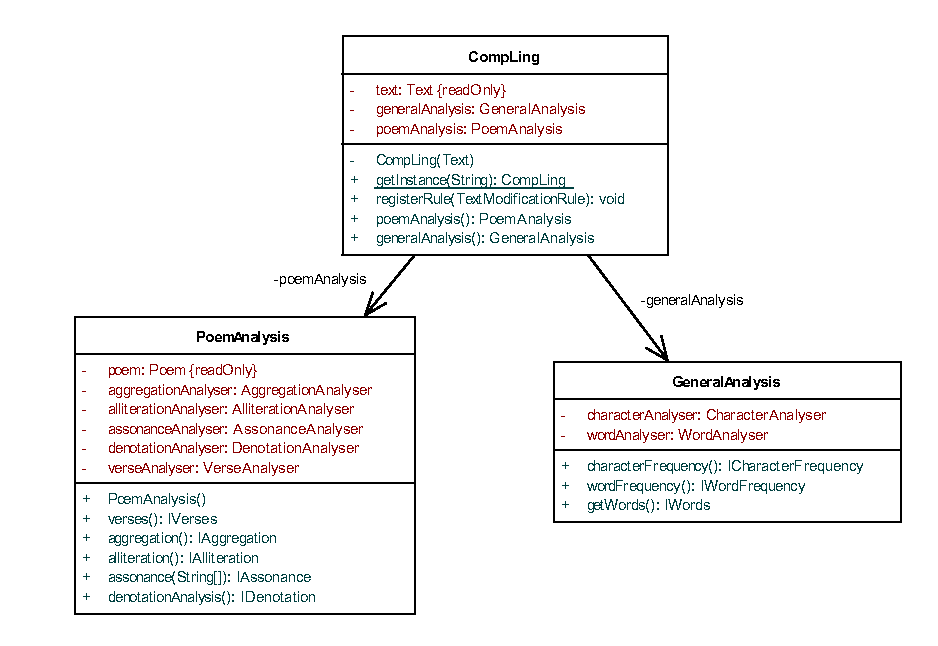
\includegraphics[max width=\textwidth,keepaspectratio=true]{imgs-60-aplikace/compLing-class-diagram.pdf}
	\caption{Diagram tříd jádra knihovny \texttt{compLing}.}
	\label{fig:compling-core-class}
\end{figure}

\section{Grafické uživatelské rozhraní}

Modul grafického uživatelského rozhraní vznikl jako nutná nadstavba nad knihovnou \texttt{compLing}, neboť knihovna sama neposkytuje žádnou jinou možnost použití (např. pomocí příkazové řádky) než \acrshort{api} a je tedy nutné začlenit ji do jiného softwarového modulu.

Cílem bylo vytvořit co možná nejjednodušší rozhraní, které uživateli umožní otevřít libovolný počet textů a následně nad těmito texty provádět analýzy podporované knihovnou \texttt{compLing}. Uživatelské rozhraní programu s 18 otevřenými překlady básně Havran je zobrazeno na následujícím obrázku:

\begin{figure}[H]
	\centering
	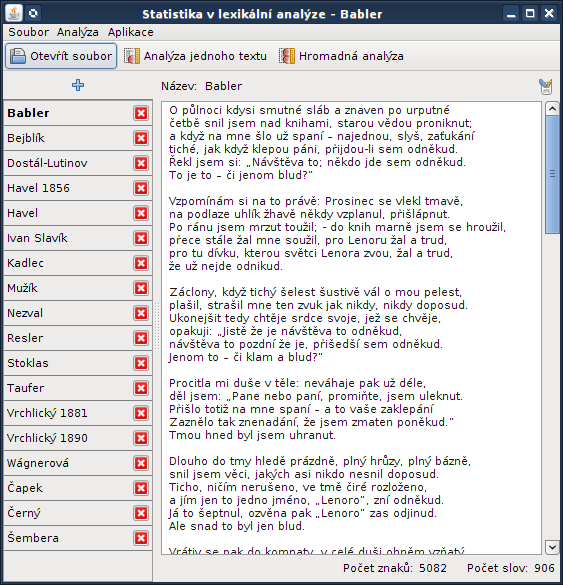
\includegraphics[max width=\textwidth,keepaspectratio=true] {imgs-60-aplikace/gui-main-window}
	\caption{Hlavní okno programu s otevřenými překlady básně Havran.}
	\label{fig:gui-main-window}
\end{figure}

Hlavní okno je rozděleno do čtyř částí:

\begin{enumerate}
	\item menu,
	\item panel nástrojů
	\item panely otevřených textů,
	\item aktuální text.
\end{enumerate}

Menu aplikace obsahuje tři položky -- \menu{Soubor}, \menu{Analýza} a \menu{Aplikace}. V menu \menu{Soubor} se nacházejí položky pro vytvoření nového prázdného panelu, otevření souboru, uložení aktuálního textu a ukončení aplikace. Menu \menu{Analýza} zpřístupňuje jednotlivé type analýz (kvantitativní, fonické, denotační). V případě, že není otevřen žádný text, je tato položka neaktivní. V menu \menu{Aplikace} se skrývají dvě položky -- \menu{Nastavení} a \menu{O aplikaci}. Položka \menu{Nastavení} vyvolá dialog, který umožňuje upravit velikost písma v aplikaci.

Panel nástrojů poskytuje rychlý přístup k nejčastěji využívaným funkcím. Těmi jsou otevírání textů, analýza aktuálního textu a analýza všech otevřených textů. Po kliknutí na tlačítko \menu{Analýza jednoho textu} nebo \menu{Hromadná analýza} je zobrazeno menu pro výběr konkrétního typu analýzy. Obě tato tlačítka jsou neaktivní, není-li otevřen žádný text.

Pod panelem nástrojů vlevo jsou ve sloupci umístěny panely pro otevřené texty. Na vrcholu panelů se nachází tlačítko pro vytvoření nového prázdného panelu. Po kliknutí pravým tlačítkem myši na panel se zobrazí kontextové menu, přes které je možné panel přejmenovat,  uložit, znovu načíst nebo uzavřít.

Nalevo od těchto panelů je zobrazen právě aktivní text. Nad i pod textem jsou umístěny dva informační panely. Vrchní zobrazuje jméno aktivního textu. Kliknutím na tlačítko vpravo (ikonka tužky) je možné text přejmenovat. Na panelu umístěném pod textem je zobrazena informace o délce aktuálního textu, a to jak v počtu znaků, tak v počtu slov.

\section{Práce s aplikací}

Tato kapitola obsahuje popis funkcí aplikace včetně ukázek, jak tyto funkce využívat. Přestože se aplikace snaží být co nejvíce uživatelsky přívětivá, ne všechny funkce mohou být na první pohled zcela zřejmé.

\subsection{Spuštění aplikace}

Spustitelná aplikace je součástí elektronické přílohy této diplomové práce. Na přiloženém CD je umístěn soubor \texttt{CompLingGui.jar}. Tento soubor je vhodné zkopírovat z CD na pevný disk počítače, na kterém má být aplikace spuštěna. Aplikaci lze spustit poklepáním na ikonu souboru \texttt{CompLingGui.jar}. Nastat mohou tři situace:

\begin{enumerate}
\item aplikace se spustí,
\item spustí se jiná aplikace (typicky archivační program, např. WinZip),
\item operační systém nemá pro soubor \texttt{jar} nastavenu žádnou asociaci a zobrazí dialog:
\end{enumerate}

\raggedbottom

\begin{figure}[H]
	\centering
	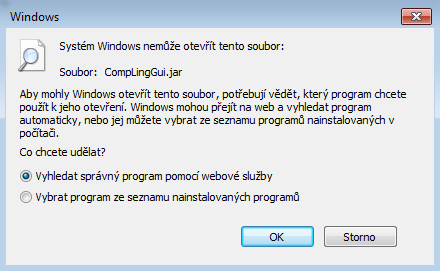
\includegraphics[max width=\textwidth,keepaspectratio=true] {imgs-60-aplikace/no-association}
	\caption{Žádná asociace pro soubory typu \texttt{jar} nenastavena.}
	\label{fig:no-association}
\end{figure}

V případě, že nastane první situace, je vše v pořádku. V opačném případě je třeba operačnímu systému říci, že má soubory typu \texttt{jar} spouštět programem \texttt{Java}. Ten již může být na počítači nainstalovaný z dřívějška, ale může se stát, že vůbec nainstalovaný není.

Pokud nastala druhá situace, tj. spustil se jiný program, než ten z obrázku ~\ref{fig:gui-main-window}, uzavřete jej, zkuste na ikonku souboru \texttt{CompLingGui.jar} kliknout pravým tlačítkem myši. Objeví se kontextové menu. Pokud menu obsahuje položku \menu{Otevřít v programu $\kern 10pt\triangleright$}, a v podmenu této položky je na výběr \menu{Java(TM)}, zvolte tuto možnost. Nyní by se měla aplikace spustit.

V případě, že Java nainstalovaná není, je třeba ji nejprve stáhnou z internetových stránek \url{https://java.com/en/download/} a poté nainstalovat. Instalátor by měl sám zajistit asociaci souborů typu \texttt{jar} s Javou. Po skončení instalace je vhodné restartovat počítač. Po restartu je možné aplikaci spustit dvojklikem na ikonu souboru \texttt{CompLingGui}.

\subsection{Práce s texty}

Po spuštění je zobrazeno hlavní okno grafického uživatelského rozhraní aplikace. Protože zatím není otevřen žádný text, je funkcionalita programu omezena o možnost provádění analýz. Pro to, aby se analyzování zpřístupnilo, je třeba vytvořit nový nebo upravit existující text.

Pro vytvoření nového prázdného textu je třeba pomocí tlačítka \menu{\ding{58}} nejprve vytvořit nový panel (eventuálně je možné pro vytvoření panelu použít menu \menu[,]{Soubor,Nový prázdný panel}). Aplikace poté vyzve k zadání jména pro nový text. Jméno textu nemůže zůstat prázdné. Do nového panelu je možné vepsat nebo vložit vlastní text. Ten může být uložen buď pomocí menu \menu[,]{Soubor,Uložit}, nebo přes kontextové menu, které je vyvoláno po kliknutí pravým tlačítkem myši na panel.

Další možností je otevřít již existující textový soubor (soubor s příponou \texttt{txt}). To je možné provést buď pomocí menu \menu[,]{Soubor,Otevřít}, nebo tlačítkem \menu{Otevřít soubor} na panelu nástrojů. Po zvolení jedné z možností se zobrazí dialog pro výběr souboru. Je možné otevřít více textů najednou označením více souborů pomocí klávesy \keys{\ctrl} a levého tlačítka myši. Pro každý z otevřených souborů je vytvořen nový panel, který je pojmenován stejně jako otevíraný soubor.

Je-li text změněn, objeví se za jeho jménem na panelu znak \texttt{*}. Změněný text je možné uložit (buď v kontextovém menu vyvolaném kliknutím pravého tlačítka myši na panel nebo v menu \menu{Soubor}), případně jej lze, je-li text načten ze souboru, znovu načíst a vrátit jej tak do původní podoby. Tato možnost je přístupná přes kontextové menu příslušného panelu (\menu[,]{klik pravým tlačítkem na panel,Nahrát znovu}).

Otevřené texty je možné uzavřít buď kliknutím na uzavírací tlačítko \menu{\ding{54}}, které se nachází na panelu vpravo, nebo přes \menu[,]{kontextové menu, Zavřít}. Aplikace zobrazí varování v případě, že byl text před uzavřením změněn a není uložen. Stejně tak je varování zobrazeno, pokud je aplikace ukončena a jsou v ní otevřené texty, které byly změněny a dosud nejsou uloženy.
\end{document}